\section{Non-normal Data}

\begin{frame}

  \begin{center}
    {\bf Non-normal Data}
  \end{center}

\end{frame}

\begin{frame}{Non Normality}{What is non-normality?}
  \begin{itemize}
    \item Until now we studied methods which {\bf assume} that the experimental
      data follows a normal distribution (or close enough).\bigskip
    \item In many cases, this assumption {\bf does not hold}. In this condition,
      how can we perform the statistical analysis of the results?
  \end{itemize}
\end{frame}

\subsection{Motivation Example}

\begin{frame}[fragile]{Non Normal data makes everything go wrong}{Weight Loss Example}
A researcher is examining two different diets, {\bf Diet A} and {\bf Diet B},
and wants to compare the weight loss by people following one diet or the other.
They obtained the following data:

\begin{verbatim}
diet.a <- c(4,3,0,-3,-4,-5,-11,-14,-15,-300)
diet.b <- c(-8,-10,-12,-16,-18,-20,-21,-24,-26,-30)
\end{verbatim}
\bigskip

As you can see, Diet A has one big outlier\footnote{Why does this outlier exist? Data input error? Very rare case?} that makes the data not normal. How much does this affect the statistical test?
\end{frame}

\begin{frame}{Non Normal data makes everything go wrong}{Weight Loss Example}
  \begin{columns}
    \column{.5\textwidth}
    Data with Outlier\\
    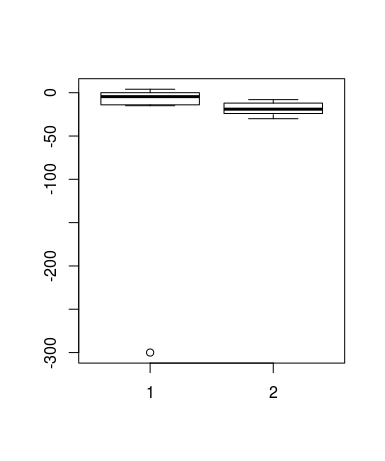
\includegraphics[width=.8\textwidth]{../img/diet_outlier1}
    \column{.5\textwidth}
    Data without Outlier\\
    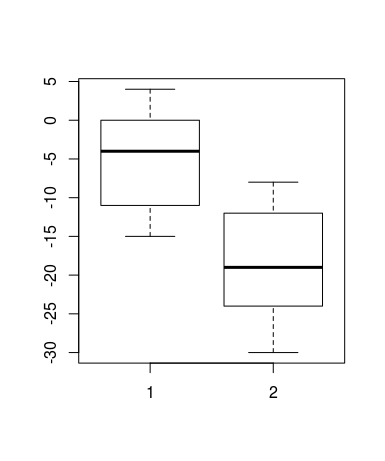
\includegraphics[width=.8\textwidth]{../img/diet_outlier2}
  \end{columns}\bigskip

  Checking a visualization, it seems like diet A has smaller losses than diet B
  overall. Except for that outlier. What happens with the T-test?
\end{frame}

\begin{frame}[fragile]{Non Normal data makes everything go wrong}{Weight Loss Example}
The standard T-test does not indicate a difference between these samples,
and even suggests that the mean of the first sample is lower!\bigskip

{\smaller
\begin{verbatim}
diet.a <- c(4,3,0,-3,-4,-5,-11,-14,-15,-300)
diet.b <- c(-8,-10,-12,-16,-18,-20,-21,-24,-26,-30)
t.test(diet.a,diet.b)

##  Welch Two Sample t-test
##
## data:  diet.a and diet.b
## t = -0.53945, df = 9.1048, p-value = 0.6025
## alternative hypothesis: true difference in
##                         means is not equal to 0
## 95 percent confidence interval:
##  -82.9774  50.9774
## sample estimates:
## mean of x mean of y
##     -34.5     -18.5
\end{verbatim}}
\end{frame}



\begin{frame}{Non Normal data makes everything go wrong}{Weight Loss Example}
\begin{columns}
  \column{.5\textwidth}
  Data with Outlier\\
  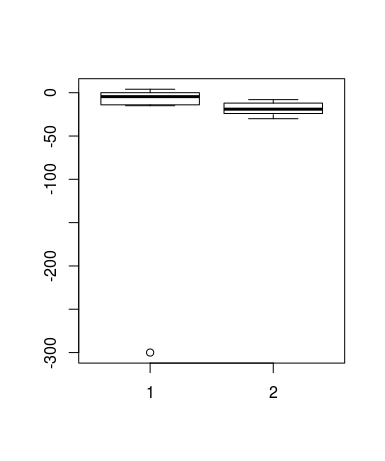
\includegraphics[width=.8\textwidth]{../img/diet_outlier1}
  \column{.5\textwidth}
  Data without Outlier\\
  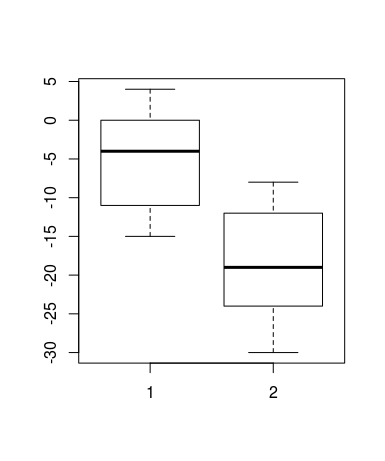
\includegraphics[width=.8\textwidth]{../img/diet_outlier2}
\end{columns}

Remember that outliers are not always this obvious!
\end{frame}


\begin{frame}[fragile]{Non Normal data makes everything go wrong}{Weight Loss Example}
Using a {\bf non-parametric test} solves the problem.

{\small
\begin{verbatim}
diet.a <- c(4,3,0,-3,-4,-5,-11,-14,-15,-300)
diet.b <- c(-8,-10,-12,-16,-18,-20,-21,-24,-26,-30)
wilcox.test(diet.a,diet.b)

##  Wilcoxon rank sum test
##
## data:  diet.a and diet.b
## W = 82, p-value = 0.01469
## alternative hypothesis: true location shift
## is not equal to 0
\end{verbatim}}
\end{frame}

\subsection{Concepts and Examples}

\begin{frame}{Non Normality}{Examples of Non Normal data?}
  There are many different ways that data can violate the assumption of normality:

  \begin{itemize}
    \item \emph{Special Data Cases: Outliers and Limits}: We saw one example of outlier that challenges the assumption of normalty. Limits in the data (minimum time) can have a similar effect.\bigskip

    \item \emph{Extreme Non-Normal Distributions.} Power Distribution, Cauchy Distribution, etc.\bigskip

    \item \emph{Ordinal Data.} Ordinal data is numeric, in the sense
    that it can be compared/ordered, but you can't rely on direct algebra.
    (eg: Human opinion scales)\bigskip

    \item \emph{Non-numerical data}: categorical data, class data, etc;
  \end{itemize}
\end{frame}


\begin{frame}{Non Normality}{Example: Random Processes} % TODO: Expand on this example

  Random processes in nature (such as plant growth or shell formation) very
  often follow a normal distribution (or bell curve). However, random artificial
  processes do not always follow a normal distribution: \bigskip

  \begin{itemize}

    \item Random numbers in computer very often use {\bf Uniform distributions}.
    (Uniform distributions can be easily approximated to normal distributions
    by the use of bootstrapping).\bigskip

    \item Random numbers from social processes very often show {\bf Power
    distributions}. Power distributions are characterized by "90\% of observations
    have 10\% of values". Examples: Salary data, Social network data, etc.

  \end{itemize}
\end{frame}

\begin{frame}{Non Normality}{Example: Likert Data} % TODO: Expand on this example

\emph{Likert} data is often collected from surveys and interview questions. It
is usually  composed of multiple questions with 5 or 7 options, ranged from
"Strongly Agree" to "Strongly Disagree", or "Always" to "Never".\bigskip

\begin{center}
  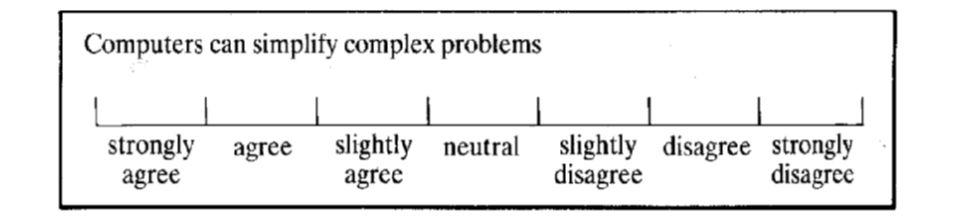
\includegraphics[width=0.9\textwidth]{../img/likert_scale}
\end{center}

Why can't we treat likert data directly as numerical?
\begin{itemize}
  \item Values outside of the 0-5 range have no meaning;
  \item Algebra on likert data has no meaning (Neutral+Disagree=?)
  \item The difference between levels is not clear. Is "Agree" equally
  distant from "Slightly Agree" and "Neutral"?
\end{itemize}
\end{frame}

% \begin{ftstf}{Non Normality}{Example: Fully Symbolic Data}
% TODO: Expand on this example
%   Some data may not have a clear numerical correspond
% \end{ftstf}


\begin{frame}{Non Normality}{Strategies for non normal data}
  Let's discuss three things that we can do about non-normal data,
  regarding statistical testing:\bigskip

  \begin{itemize}
    \item Do nothing
    \item Transform the Data
    \item Non parametric Testing
  \end{itemize}\bigskip

  Please note that this is a quick overview of the treatment of non-normal data.
  {\bf Study your particular case carefully!}
\end{frame}

% TODO: DO NOTHING SECTION
%    - remove outliers
%    - Trusting the CLT
%    - You need to understand WHY your data is not normal ()
% TODO: How to report on non-normal data
% TODO: FIXME: separate the lecture in *skewed* data and *ordinal* data.
% \begin{ftstf}{Non Normality}{Reporting on non-normal data} %% What you need to write on the paper
%   \begin{itemize}
%     \item Mean, Median, Ranks
%     \item Standard Deviation and IQR
%   \end{itemize}
% \end{ftstf}
%
% TODO: When is it ok to ignore small violations of normality?
% \section{Do nothing}
%
% \begin{ftstf}{Strategy 1 - Do nothing}{Ignoring the assumption of normality.}
%   \begin{itemize}
%     \item Very high number of samples is available (how high?);
%     \item The other conditions must still hold;
%   \end{itemize}
% \end{ftstf}
% TODO: R-code: some normal data with high n do not pass a normality test.
% findNonNormal <- function(n = 5000){
%     p <- 1
%     while(p > 0.05) {
%         y <- rnorm(n)
%         p <- shapiro.test(y)$p.value
%         }
%     y
%     }
%
% y <- findNonNormal()
% hist(y)
% qqnorm(y)


\section{Data Transformation}

\begin{frame}{Data Transformation}{Log Transformation}
  We can apply certain transformations to "normalize" some data.
  \begin{center}
    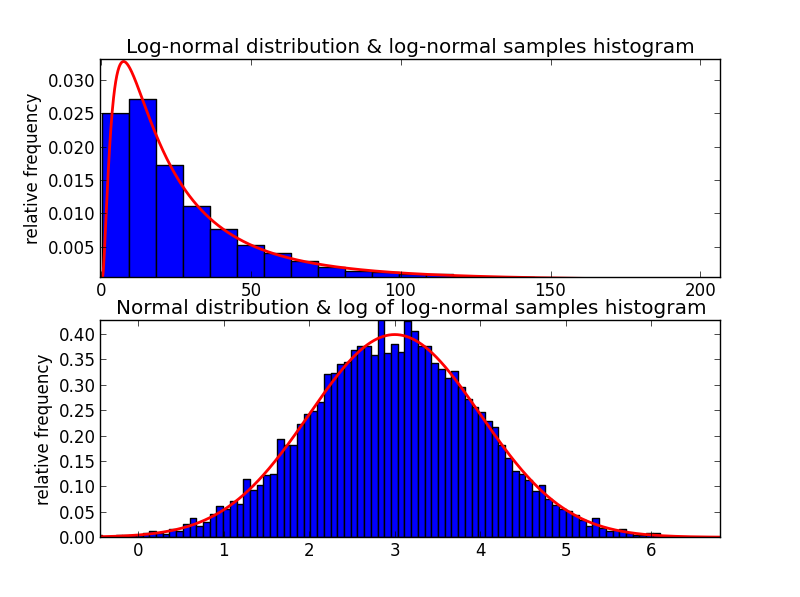
\includegraphics[width=0.75\textwidth]{../img/lognormal_transformation}
  \end{center}
\end{frame}

%% TODO: Add images here
\begin{frame}[fragile]{Log Transformation}{}
\begin{verbatim}
# Generate lognormal data
#
set.seed(17)
z <- exp(rnorm(200, -2, 0.4))

# Log transformation
#
y <- log(z)
mu.hat <- mean(y)
sigma.hat <- sd(y)
\end{verbatim}
\end{frame}

\begin{frame}{Data Transformation}{Other transformations}
  \begin{itemize}
    \item For left skewed data:
    \begin{itemize}
      \item square root, cube root, log
    \end{itemize}
    \item For right skewed data:
    \begin{itemize}
      \item square root (constant $-x$), cube root (constant $-x$)
    \end{itemize}
  \end{itemize}\bigskip

  Attention: Logarithm of 0 and negative data is not defined, so you may need to
  add a constant before the transformation.
\end{frame}




\begin{frame}{Data Transformation}{Be careful when transforming data}
  \begin{itemize}
    \item Careful when reporting back the data on the paper.
    \begin{itemize}
      \item Make sure to mention what data transformation was used in the analysis.
      \item Apply {\bf back-transformation} before discussing results.
    \end{itemize}\bigskip

    \item Beware of when Null hypotheses are not equivalent!
    \begin{itemize}
      \item Example: Lognormal mean includes the variance. Transformed lognormal mean does not. Null hypothesis is only equivalent when variance is equal!
    \end{itemize}
  \end{itemize}
\end{frame}


\subsection{Bootstrapping}

\begin{frame}{Bootstrapping}{}
  Another way to make data follow a normal distribution is to use
  the {\bf Bootstrapping} procedure. Bootstrapping uses the idea of the CLT
  (central limit theorem) by creating a "sample mean distribution" that
  will usually follow the normal distribution.
\end{frame}

\begin{frame}{Bootstrapping}{The Bootstrapping Procedure}
  \begin{itemize}
    \item Take $n$ samples of size $m$ (with repetition)
    \item Calculate the mean of each sample.
    \item Your bootstrapped data is the set of sample means.

    \begin{center}
      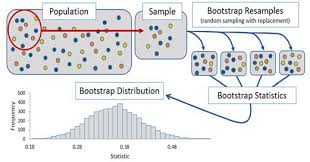
\includegraphics[width=.8\textwidth]{../img/bootstrap_lowres}
    \end{center}
  \end{itemize}

  % TODO: Code Example
\end{frame}

\begin{frame}{Bootstrapping}{Using Bootstrapped Data}
  The R package "boot" can help you appropriate create tests
  and confidence intervals from bootstrapped data.
\end{frame}

\section{Non-Parametric Tests}

\begin{frame}{Non Parametric Tests}{}
  Non-parametric tests remove the assumption of normality from the
  population distribution. On the other hand, they can be a bit weaker, and
  cannot estimate the real-world distance between two samples.
  \bigskip

  \begin{itemize}
    \item Wilcoxon Signed Rank Test (1 sample)
    \item Wilcoxon Ranked Sum Test / Mann-whitney Test (2 samples)
    \item Kruskall-Wallis Test (multiple samples)
  \end{itemize}
\end{frame}

% \begin{frame}{Non Parametric Tests}{Basic Idea}
%   % TODO: Generally explain the basic idea of non-parametric tests
% \end{frame}

\subsection{1 or 2 samples}

\begin{frame}{Non Parametric Tests}{One or two Samples}
  \begin{itemize}
    \item unpaired test: Mann-Whitney U-test;
    \item paired test: Wilcoxon signed-ranks test;
  \end{itemize}
\end{frame}

\begin{frame}{Mann-Whitney U-test}{}
  \begin{center}
    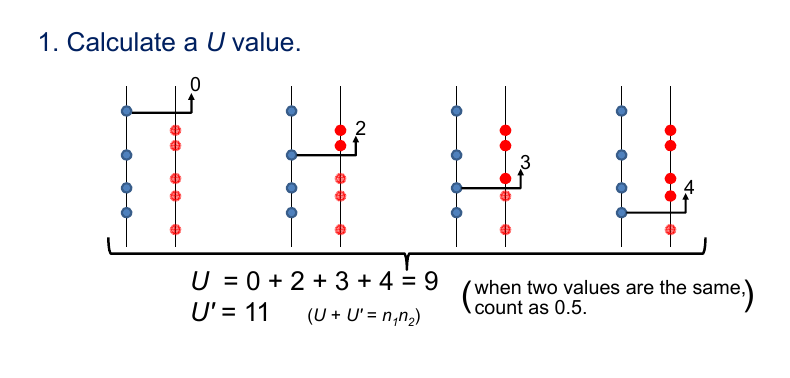
\includegraphics[width=1\textwidth]{../img/MannWhitneyU}
  \end{center}
\end{frame}

\begin{frame}{Mann-Whitney U-test}{}
  \begin{center}
    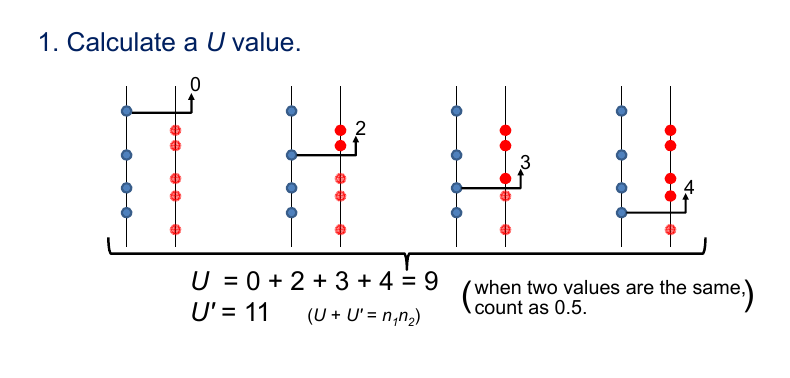
\includegraphics[width=.6\textwidth]{../img/MannWhitneyU}
  \end{center}

  \begin{itemize}
    \item Choose the smaller value of U or U'
    \item Null Hypothesis: {\bf Both samples come from the same distribution}
    \item Under the null hypothesis, for big enough $n_1$ and $n_2$, U follows
    roughly a normal distribution with mean $\frac{n_1n_2}{2}$ and variance $\frac{n_1n_2(n_1+n_2+1)}{12}$
    \item Calculate the test statistic z, and find the p-value from the $\alpha$-percentile in the z distribution.
  \end{itemize}
\end{frame}

\begin{frame}{Wilcoxon Signed Rank Test}{}
  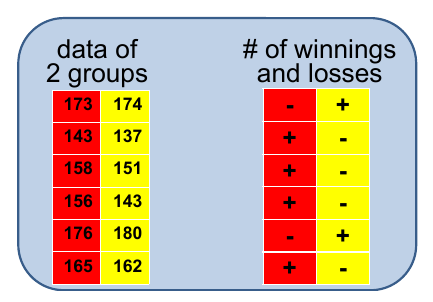
\includegraphics[width=.4\textwidth]{../img/SignTest}

  \begin{itemize}
    \item The Wilcoxon test takes the relative difference between pairs (positive or negative)
    \item Null hypothesis: {\bf Positive and Negative signs are equally likely}
    \item The overall number of signs is compared against a binomial distribution under the Null hypothesis.
  \end{itemize}
\end{frame}


\begin{frame}[fragile]{Wilcoxon Signed Rank Test}{R example}

{\smaller
\begin{verbatim}
## Hollander & Wolfe (1973), 29f.
## Hamilton depression scale factor measurements in 9
## patients with mixed anxiety and depression, taken at
## the first (x) and second (y) visit after initiation
## of a therapy (administration of a tranquilizer).

x <- c(1.83,  0.50,  1.62,  2.48, 1.68, 1.88,
       1.55, 3.06, 1.30)
y <- c(0.878, 0.647, 0.598, 2.05, 1.06, 1.29,
       1.06, 3.14, 1.29)

wilcox.test(x, y, paired = TRUE, alternative = "greater")

Wilcoxon signed rank test
data:  x and y
V = 40, p-value = 0.01953
alternative hypothesis: true location shift
is greater than 0
\end{verbatim}}
\end{frame}

%% TODO: Move this to the multiple samples (ANOVA) lecture
% \subsection{Multiple Samples}
%
% \begin{ftstf}{Non Parametric Tests}{Multiple Samples}
%   \begin{itemize}
%     \item unpaired test: Kurskal-Wallis test
%     \item paired test: Friedman test
%   \end{itemize}
% \end{ftstf}
